%%%%%%%%%%%%%%%%%%%%%%%%%%%%%%%%%%%%%%%%%%%%%%%%%%%%%%%%%%%%%
%% Begin exercise %%
%%%%%%%%%%%%%%%%%%%%%%%%%%%%%%%%%%%%%%%%%%%%%%%%%%%%%%%%%%%%%
\ex{Step-up and (synchronous) buck-boost converters}


%%%%%%%%%%%%%%%%%%%%%%%%%%%%%%%%%%%%%%%%%%%%%%%%%%%%%%%%%%%%%
%% Task 1: Boost Converter with no losses %%
%%%%%%%%%%%%%%%%%%%%%%%%%%%%%%%%%%%%%%%%%%%%%%%%%%%%%%%%%%%%%
\task {Boost converter with no losses}
The boost converter which is shown in \autoref{fig:boost converter with no losses} supplies a resistive load with a rated voltage of $U_{\mathrm{2}} = \SI{60}{\volt}$. The converter operates in steady state and all losses of the boost converter are neglected.

\begin{figure}[htb]
    \begin{center}
        
    %\begin{tikzpicture}
    \begin{circuitikz}[european currents,european resistors,american inductors]
        \draw
        (0,0) coordinate(u1o)
        to [V,v_=$U_1$] ++(0,-3) coordinate(u1u)
        (0,0) to[R, l=$R_L$] (2.5,0)
        (2.5,0) to[L, l=$\mathrm{L}$] (4.5,0)

        (4,0) coordinate(N1) to [short] ++(1.5,0) coordinate(Ud)
        ++(0,-1.5) node[nigfete](Trans){}
        (Ud) to [short] (Trans.drain)
        (Trans.source) to [short,-] ++(0,0) coordinate(U2p)
      
        (4,0) to [short,-] (9.5,0)

        (5.5,-1.5) to [short,-] ++(0,-1.5) 

        (6.5,0) to[D, l=$D$] (8,0)
                
        (8,0) to[C,l_=$C$] (8,-3)

        (9.5,0) to [R,l_=$R$,v^=$U_\text{2}$,voltage shift=0.5, voltage=straight] (9.5,-3)

        (9.5,-3) to [short,-] (0,-3)

        (0.75,0) to [short,i^<=$i_1$(t)] (u1o)
        (4.5,0) to [short,-*,i^>=$i_L$(t)] (5.5,0)
        
        (5.5,-0.5) to [short,i^<=$i_\mathrm{T}$(t)] (5.5,-1)
        
        (9,0) to [short,i^<=$I_2$(t)] (8.5,0)
        ;
% (u3o) to [short,-] ++(1,0) coordinate(v1)
        ;
    \end{circuitikz}
    \caption{Boost converter}
     \label{fig:boost converter}
\end{center}
%\end{tikzpicture}
\end{figure}


The specification of the boost converter is given in \autoref{table:ex02_Parameters of the circuit}.

\begin{table}[ht]
    \centering  % Zentriert die Tabelle
    \begin{tabular}{llll}
        \toprule
        
        Input voltage: &  $U_{\mathrm{1}} = \SI{12}{\volt}$ & Output voltage: & $U_{\mathrm{2}} = \SI{60}{\volt}$ \\ 
        Output current: & $I_2 = \SI{2}{A}$  & Minimal output power: & $P_{\mathrm{2,min}} = \SI{10}{\watt}$ \\ 
        Output voltage ripple: & $\triangle u_{\mathrm{2}} = \SI{120}{\milli\volt}$  & Switching frequency: & $f_{\mathrm{s}} = \SI{100}{\kilo\hertz}$ \\ 
        \bottomrule
    \end{tabular}
    \caption{Parameters of the boost converter.}  % Beschriftung der Tabelle
    \label{table:ex02_Parameters of the circuit}
\end{table}
%
\subtask{Derive the duty cycle $D$ which leads to the specific output voltage of $U_{\mathrm{2}} = \SI{60}{\volt}$.}

\begin{solutionblock}
    \begin{solutionfigure}[ht]
    \centering
    \begin{tabular}{cc}
        ECD $T_{\mathrm{s,on}}$ & ECD $T_{\mathrm{s,off}}$\\
        \begin{circuitikz}[european currents,european resistors,american inductors,]
            \draw
            (0,0) coordinate(u1o)
            to [V,v^=$U_2$] ++(0,-3) coordinate(u1u)
            (u1o) to [short,-] ++(-0.25,0) coordinate(o)
            (u1u) to [short,-] ++(-1,0) coordinate(u2u)
            (u2u) to [short,-,v^<=$u_\text{s}$,mirror,voltage=straight] ++(0,3) coordinate(u2o)
            (u2o) to [short,-] ++(0.25,0) coordinate(u) ++ (-3.5,0) coordinate(u3o)
            (u3o) to [V,v_=$U_1$] ++(0,-3) coordinate(u3u)
            (u3u) to [short,-] ++(3.5,0) coordinate(t)
            
            (u3o) ++(+2,0) to [L,l_=$L$,v^<=$u_\text{L}(t)$,mirror,voltage=straight]   
             ++(-1,0) coordinate(uqo)
            (u3o) to [short,-] ++(1,0) coordinate(v1)
            (u2o) to [short,-] ++(-1.15,0) coordinate(v2)
            (u2o) to [short,-,i^<=$i_L$(t)] ++(-1,0)
            ;
        \end{circuitikz} 
    &
    
        \begin{circuitikz}[european currents,european resistors,american inductors,]
            \draw
            (0,0) coordinate(u2o)
            to [V,v^=$U_2$, voltage=straight] ++(0,-3) coordinate(u2u)
                (u2o) to [short,-,i^<=$i_L$(t)] ++(-1,0) to [L,l_=$L$,v^<=$u_\text{L}(t)$,mirror,voltage=straight] ++(-3,0) coordinate(Ll) ++(-1,0) coordinate(uqo)
                (-4,0) to [V,v_=$U_1$] ++(0,-3) coordinate(u2u)
                (-4,-3)  to [short,-] ++(4,0) coordinate(r)
                ;
        \end{circuitikz}
    \end{tabular}
    \caption{ECD of the boost converter for different switching states.}
    \label{fig:switching_states_step-down_converter}
\end{solutionfigure}
    The equivalent circuit diagram (ECD) is shown in \autoref{fig:switching_states_step-down_converter}.
    As there are no losses at the transistor, the voltage $U_{\mathrm{1}}$ is equal to $u_{\mathrm{L}}$ for the switch-on period $T_{\mathrm{on}}$ and is defined as
    \begin{equation}
        U_{\mathrm{1}} = u_{\mathrm{L}} = L \frac{\Delta i_{\mathrm{L}} }{\Delta t}. 
    \end{equation}
    This subtask does not consider the complete period $T_{\mathrm{s}}$, but only the switch-on period $T_{\mathrm{s,on}}$. Furthermore, the initial state of the current $i_{\mathrm{L}}$ must also be considered.
    That is why we can completely rearrange the equation into:
    \begin{equation}
        i_{\mathrm{L}}(T_{\mathrm{s,on}}) =  \frac{U_{\mathrm{1}} }{L}T_{\mathrm{s,on}} +  i_{\mathrm{L}}(0).
    \end{equation}
    Applying Kirchhoff's second law, the voltage equation for the  the switch-off time $T_{\mathrm{s,off}}$ is given with:
    \begin{equation}
        U_{\mathrm{1}} = u_{\mathrm{L}} + U_{\mathrm{2}}.
    \end{equation}
    Now, the differential expression for $u_{\mathrm{L}}$ leads to:
    \begin{equation}
        L \frac{\Delta i_{\mathrm{L}} }{\Delta t} = U_{\mathrm{1}} - U_{\mathrm{2}}.
    \end{equation}
    The equation for the current $i_{\mathrm{L}}$ at the switch-off time $T_{\mathrm{s,off}}$ results from the term describing the discharge of the inductance from $T_{\mathrm{s,off}}$ together with the initial condition of the current at this time
    \begin{equation}
        i_{\mathrm{L}}(t) = \frac{U_{\mathrm{1}}-U_{\mathrm{2}} }{L} (t-T_{\mathrm{s,on}})+i_{\mathrm{L}}(T_{\mathrm{s,on}}).
    \end{equation}
    This results in the equation for the entire current curve over the period: 
    \begin{equation}
        i_{\mathrm{L}}(t) = \frac{U_{\mathrm{1}}-U_{\mathrm{2}} }{L} (t-T_{\mathrm{s,on}})+\frac{U_{\mathrm{1}}}{L}T_{\mathrm{s,on}}+i_{\mathrm{L}}(0).
    \end{equation}
    If you now consider the steady state $i_{\mathrm{L}}(t=0)=i_{\mathrm{L}}(t=T_{\mathrm{s}})$, this results in the following:
    \begin{equation}
        i_{\mathrm{L}}(0) = \frac{U_{\mathrm{1}}-U_{\mathrm{2}} }{L} (T_{\mathrm{s,off}})+\frac{U_{\mathrm{1}}}{L}T_{\mathrm{s,on}}+i_{\mathrm{L}}(0).
    \end{equation}
    Now the initial condition $i_{\mathrm{L}}(0)=0$ is assumed as 
    \begin{equation}
        0 = \frac{U_{\mathrm{1}}-U_{\mathrm{2}} }{L} (T_{\mathrm{s,off}})+\frac{U_{\mathrm{1}}}{L}T_{\mathrm{s,on}}.
    \end{equation}
    Canceling out the inductance leads to
    \begin{equation}
        U_{\mathrm{1}}T_{\mathrm{s,on}}= (-U_{\mathrm{1}}+U_{\mathrm{2}})T_{\mathrm{s,off}},
    \end{equation}
    rearranging the time results into:
    \begin{equation}
        U_{\mathrm{1}}(T_{\mathrm{s,off}}+T_{\mathrm{s,on}})=  U_{\mathrm{2}}T_{\mathrm{s,off}}.
    \end{equation}
    The switch-off period $T_{\mathrm{s,off}}$ plus the switch-on period $T_{\mathrm{s,on}}$ is the total period $T_{\mathrm{s}}$. The following equation can now be established for the duty cycle:
    \begin{equation}
        \frac{U_{\mathrm{1}}}{U_{\mathrm{2}}}= \frac{T_{\mathrm{s,off}}}{T_{\mathrm{s}}}= \frac{T_{\mathrm{s}}}{T_{\mathrm{s}}}-\frac{T_{\mathrm{s,on}}}{T_{\mathrm{s}}} = 1-D.
    \end{equation}
    And with the values given in the task, the duty cycle is calculated as follows:
    \begin{equation}
        D = 1-\frac{U_{\mathrm{1}}}{U_{\mathrm{2}}} = 1- \frac {\SI{12}{\volt}} {\SI{60}{\volt}} = 0.8.
    \end{equation}
\end{solutionblock}


\subtask{Determine the average input current $\overline i_{\mathrm{L}}$.}
\begin{solutionblock}
    With neglecting the losses $(P_{\mathrm{l}} = \SI{0}{\watt})$ of the boost converter and assuming a good smoothing of the inductor current, the average value $\overline i_{\mathrm{L}}$ is equal $I_{\mathrm{1}}$ and can be calculated using the power balance
    \begin{equation}
        P_{\mathrm{2}} = U_{\mathrm{2}} I_{\mathrm{2}} = {\SI{60}{\volt}} \cdot {\SI{2}{\ampere}} = {\SI{120}{\watt}}.
    \end{equation}
    Since no losses are taken, the power  $P_{\mathrm{1}}$ is equal to  $P_{\mathrm{2}}$.
    This results in the average current $\overline i_{\mathrm{L}}$:
    \begin{equation}
         I_{\mathrm{1}} = \overline i_{\mathrm{L}} = \frac{P_{\mathrm{1}}}{U_{\mathrm{1}}}= \frac{\SI{120}{\watt}}{\SI{12}{\volt}} = \SI{10}{\ampere}.
    \end{equation}
    An alternative solution would be to determine the average current $\overline i_{\mathrm{L}}$ via the duty cycle
    \begin{equation}
    \frac{I_{\mathrm{1}}}{I_{\mathrm{2}}}=\frac{1}{1-D}.
    \end{equation}
    \begin{equation}
     I_{\mathrm{1}}=\frac{I_{\mathrm{2}}}{1-D}=\frac{\SI{2}{\ampere}}{1-0.8}= \SI{10}{\ampere}.
    \end{equation}
\end{solutionblock}

\subtask{ Define a suitable inductance for the coil $L$, so that the boost converter is operating in boundary conduction mode (BCM) when supplying the minimum output power $P_\mathrm{2,min}$. Determine the maximal switch-off current $i_{\mathrm{T}}$ of the transistor $T$ for the rated output current $I_{\mathrm{2}} = \SI{2}{\ampere}$.}
\begin{solutionblock}
    Because no losses are assumed, $P_{\mathrm{1,min}}=P_{\mathrm{2,min}}$.
    The following equation is used to calculate the average current $I_{\mathrm{1,min}}$ over a period to achieve the minimum input power
    \begin{equation}
        I_{\mathrm{1,min}} = \frac{P_{\mathrm{1,min}}}{U_{\mathrm{1}}} = \frac{\SI{10}{\watt}}{\SI{12}{\volt}}= \SI{0.833}{\ampere}.
    \end{equation}
    The requirement for BCM is, that the current is zero at the starting point of the period  $i_\mathrm{1,BCM}(0)=\SI{0}{\ampere}$.
    Due to the triagular current waveform of the inductor current $i_{\mathrm{L}}$, the maximum current is given with:
    \begin{equation}
        i_\mathrm{1,BCM}(T_{\mathrm{s,on}})= 2I_{\mathrm{1,min}}= 2\cdot \SI{0.833}{\ampere} = \SI{1.667}{\ampere}.
    \end{equation}
    The differential equation of the inductance is defined as:
    \begin{equation}
        u_\mathrm{L}=L\frac{\mathrm{d}i_\mathrm{L}(t)}{\mathrm{d}t}.
    \end{equation}
    Neglecting saturation, the equation simplifies to:
    \begin{equation}
        u_\mathrm{L}=L\frac{\Delta i_\mathrm{L}}{\Delta t}.
    \end{equation}
    Only the switch-on period is considered, therefore $\Delta t = T_{\mathrm{s,on}}$. Furthermore, $u_\mathrm{L}=U_\mathrm{1}$ and $\Delta i_\mathrm{L} = 2 I_\mathrm{1min}$.
    The switch-on period can be determined by the known duty cycle $D$ and the known frequency $f_{\mathrm{s}}$
    \begin{equation}
        T_{\mathrm{s,on}} = D T_{\mathrm{s}} = \Delta t = \frac{D}{f_{\mathrm{s}}} = \frac{0.8}{\SI{100}{\kilo\hertz}}=\SI{8}{\micro\second}.
    \end{equation}
    The following inductivity equation can be derived from the difference quotient equation as:
    \begin{equation}
        L=\frac{\Delta t u_\mathrm{L} }{\Delta i_\mathrm{L}}= \frac{D U_\mathrm{1}}{f_{\mathrm{s}}2I_{\mathrm{1,min}}} = \frac{0.8 \cdot \SI{12}{\volt}}{\SI{100}{\kilo\hertz\cdot 2\cdot \SI{1.667}{\ampere}}} = \SI{57.6}{\micro\henry}.
    \end{equation}
    The maximum current flows through the transistor at the end of the switch-on interval
    \begin{equation}
        I_\mathrm{T,max} = \frac{\Delta I_\mathrm{L}}{2}=\frac{\SI{1.667}{\ampere}}{2} = \SI{0.833}{\ampere}.
    \end{equation}
\end{solutionblock}

\subtask{Calculate a suitable capacitance to meet the output voltage ripple specification. Determine the current stress of the capacitor $I_\mathrm{C,RMS}$.}
\begin{solutionblock}
    The reaction of the voltage fluctuation on the current fluctuation is neglected. During on-state of the transistor, the output capacitor feed the load. Assuming an constant output current and an ideal capacitor, the output can be adopted as linearly decreasing for this interval.

    The differential form of the capacitor equation is used for this task
    \begin{equation}
        i_\mathrm{C}=C \frac{\mathrm{d}u_\mathrm{c}(t)}{\mathrm{d}t}.
    \end{equation}
    Simplifications can be assumed as:
    \begin{equation}
        i_\mathrm{C}=C \frac{\Delta u_\mathrm{c}}{\Delta t}.
    \end{equation}
    In addition, $i_\mathrm{C}=I_\mathrm{2}$ and $\Delta u_\mathrm{c}=\Delta u_\mathrm{2}$.
    $\Delta t$ is again equal to the switch-on period and can be represented by the following equation
    \begin{equation}
        \Delta t = \frac{D}{f_\mathrm{s}}. 
    \end{equation}
    Now that everything is known, the capacity can be determined
    \begin{equation}
        C = \frac{I_\mathrm{2}\Delta t}{\Delta u_\mathrm{2}}= \frac{I_\mathrm{2}D}{\Delta u_\mathrm{2}f_\mathrm{s}}=\frac{\SI{2}{\ampere}\cdot 0.8}{\SI{120}{\milli\volt} \cdot \SI{100}{\kilo\hertz}}=\SI{133.333}{\micro\farad}.
    \end{equation}
     During the on-state of the transistor we can assume an constant current which discharges the capacitor. During of-state the capacitor is charge with the current $i_\mathrm{1}-i_\mathrm{2}$.The average of the capacitor current is zero. An important rule during dimensioning the capacitor is the RMS value of the current.
     The RMS value of the current is determined using the following equation
     \begin{equation}
        I_\mathrm{C}=\sqrt{\frac{1}{T_\mathrm{s}}\int_{0}^{T_\mathrm{s}}i_\mathrm{c}(t)^2\mathrm{d}t}.
     \end{equation}
     The switch-on and switch-off periods are now set
     \begin{equation}
        I_\mathrm{C}=\sqrt{\frac{1}{T_\mathrm{s}}\int_{0}^{DT_\mathrm{s}}i_\mathrm{c}(t)^2\mathrm{d}t+\frac{1}{T_\mathrm{s}}\int_{DT_\mathrm{s}}^{T_\mathrm{s}}i_\mathrm{c}(t)^2\mathrm{d}t}.
     \end{equation}
     With neglecting the current ripple (goodsmoothing):
     \begin{equation}
        I_\mathrm{C}=\sqrt{D (I_\mathrm{2})^2+(1-D)(I_\mathrm{1}-I_\mathrm{2})^2}=\sqrt{0.8\cdot (\SI{2}{\ampere})^2+(1-0.8)\cdot(\SI{10}{\ampere}-\SI{2}{\ampere})^2} = \SI{4}{\ampere}.
     \end{equation}
     The following equation is now used for the current ripple
     \begin{equation}
        I_\mathrm{C}=\sqrt{D (I_\mathrm{2})^2\left[1+\frac{1}{3}\left[\frac{\Delta i_\mathrm{L}}{2I_\mathrm{2}}\right]^2\right]+(1-D)(I_\mathrm{1}-I_\mathrm{2})^2\left[1+\frac{1}{3}\left[\frac{\Delta i_\mathrm{L}}{2(I_\mathrm{1}-I_\mathrm{2})}\right]^2\right]}
    \end{equation}
    \begin{equation}
        I_\mathrm{C}=\sqrt{0.8 \cdot (\SI{2}{\ampere})^2 \left[1+\frac{1}{3}\left[\frac{\SI{0.833}{\ampere}}{2\cdot (\SI{2}{\ampere})}\right]^2\right]+(1-0.8)(\SI{10}{\ampere}- \SI{2}{\ampere})^2\left[1+\frac{1}{3}\left[\frac{\SI{0.833}{\ampere}}{2(\SI{10}{\ampere}- \SI{2}{\ampere})}\right]^2\right]}=\SI{4.023}{\ampere}.
    \end{equation}
\end{solutionblock}

%%%%%%%%%%%%%%%%%%%%%%%%%%%%%%%%%%%%%%%%%%%%%%%%%%%%%%%%%%%%%
%% Task 2: Boost Converter with losses %%
%%%%%%%%%%%%%%%%%%%%%%%%%%%%%%%%%%%%%%%%%%%%%%%%%%%%%%%%%%%%%
\task{Boost converter with losses}
Next, the impact of power losses on the above's converter behavior is investigated. For the following points an ideal smoothed input current and a ripple-free output voltage are assumed. The boost converter with losses  is shown in \autoref{fig:boost converter with losses}.

\begin{figure}[htb]
    \begin{center}
        
    %\begin{tikzpicture}
    \begin{circuitikz}[european currents,european resistors,american inductors]
        \draw
        (-1,0) coordinate(u1o)
        to [V,v_=$U_1$] ++(0,-4) coordinate(u1u)
        (0,0) to[R, l=$R_\mathrm{L}$] (2.5,0)
        (2.5,0) to[L, l=${L}$] (4,0)

        (4,0) coordinate(N1) to [short] ++(1.5,0) coordinate(Ud)
        ++(0,-3.23) node[nigfete](Trans){}
        %(Ud) to [short] (Trans.drain)
        (Trans.source) to [short,-*] ++(0,0) coordinate(U2p)
        
        (5.5,0) to[R, l_=$R_\mathrm{T}$] (5.5,-1.9)

        (Trans) ++(-1,0) node {$T$}

        (9,0) to [short,-] (12,0)
        (12.5,-4) to [short,-] (9.5,-4)
        (11,-4) to[short,*-] ++(0,0) 

        (5.5,-1.5) to [short,-] ++(0,-1.5) 

        (5,0) to[R, l=$R_\mathrm{D}$] (7.8,0)
        (7.5,0) to[L, l=$L_\mathrm{c}$] (9.3,0)
        (9,0) to[D, l=$D$] (12,0)

        (11,0) to[short,*-] ++(0,0) % Punkt direkt hinter der Diode

        (11,0) to[C,l_=$C$] (11,-4)

        (12.5,0) to [R,l_=$R$,v^=$U_\text{2}$,voltage shift=0.5, voltage=straight] (12.5,-4)

        (9.5,-4) to [short,-] (-1,-4)

        (0.70,0) to [short,i_<=$i_1$(t)] (u1o)
        (4.5,0) to [short,-*,i^>=$i_\mathrm{L}$(t)] (5.5,0)

        (5.5,-3) to [short,i^>=$i_\mathrm{T}$(t)] (5.5,-2)

        (11,0) to [short,i^>=$i_2$(t)] (12.5,0)
        ;
\end{circuitikz}
    \caption{Boost converter with losses}
     \label{fig:boost converter with losses}
\end{center}
%\end{tikzpicture}
\end{figure}


\subtask{From now on, the influence of the resistor $R_\mathrm{L}$ is considered. Derive the efficiency $\eta$ and voltage ratio $U_\mathrm{1}/U_\mathrm{2}$ of the boost converter in dependence on the duty cycle $D$ and the resistance ratio $\alpha= R_\mathrm{L}/R$. Sketch both functions, $\eta$ and  $U_\mathrm{2}/U_\mathrm{1}$ over the duty cycle $D$ and analyze the findings.} 
\begin{solutionblock}
We are looking for: $\eta= F(D,\alpha)$ and $\frac{U_\mathrm{2}}{U_\mathrm{1}}=F(D,\alpha)$ with $\alpha=\frac{R_\mathrm{L}}{R}$
Assuming a good smoothing of the inductor current yields to $I_\mathrm{L}=\overline i_\mathrm{L}=i_\mathrm{L}(t)$
The efficiency is given by the following equation
\begin{equation}
    \eta = \frac{P_\mathrm{2}}{P_\mathrm{1}} = \frac{P_\mathrm{2}}{P_\mathrm{2}+P_\mathrm{l}} = \frac{U_\mathrm{2} I_\mathrm{2}}{U_\mathrm{2} I_\mathrm{2} +R_\mathrm{L} I_\mathrm{L}^2} \label{eq:efficiency}.
\end{equation}
If we now consider the node around $I_\mathrm{2}$, we can establish the following equation. It must be noted that the capacitor is charged and discharged when it is switched off. The same applies to the inductor, which discharges when it is switched off. The following equation can be created from these assumptions
\begin{equation}
    I_\mathrm{2}=\frac{1}{T_\mathrm{s}} \int_{0}^{DT_\mathrm{s}} i_\mathrm{C, discharg}(t)\mathrm{d}t-\frac{1}{T_\mathrm{s}} \int_{DT_\mathrm{s}}^{T_\mathrm{s}} i_\mathrm{C,charg}(t)\mathrm{d}t+\frac{1}{T_\mathrm{s}} \int_{DT_\mathrm{s}}^{T_\mathrm{s}} I_\mathrm{L}(t)\mathrm{d}t.
\end{equation}
Since it is assumed that the charging and discharging currents of the capacitor are equal, they cancel each other out
\begin{equation}
    0 = \frac{1}{T_\mathrm{s}} \int_{0}^{DT_\mathrm{s}} i_\mathrm{C discharg}(t)\mathrm{d}t-\frac{1}{T_\mathrm{s}} \int_{DT_\mathrm{s}}^{T_\mathrm{s}} i_\mathrm{C charg}(t)\mathrm{d}t.
\end{equation}
This simplifies the explanation of this expression
\begin{equation}
    I_\mathrm{2}= \frac{1}{T_\mathrm{s}} \int_{DT_\mathrm{s}}^{T_\mathrm{s}} I_\mathrm{L}(t)\mathrm{d}t.
\end{equation}
If the current $I_\mathrm{L}$ is now assumed to be independent of $t$, the integral can be solved as:
\begin{equation}
    I_\mathrm{2}= \frac{I_\mathrm{L}}{T_\mathrm{s}}(T_\mathrm{s}-(DT_\mathrm{s}))=I_\mathrm{L}(1-D).
\end{equation}
Now we insert the equation we have just calculated into equation \eqref{eq:efficiency}. This results into: 
\begin{equation}
    \eta=\frac{U_\mathrm{2}I_\mathrm{2}}{U_\mathrm{2}I_\mathrm{2}+\frac{ R_\mathrm{L}I_\mathrm{2}^2}{(1-D)^2}}=\frac{U_\mathrm{2}}{U_\mathrm{2}+\frac{ R_\mathrm{L}I_\mathrm{2}}{(1-D)^2}}=\frac{RI_\mathrm{2}}{RI_\mathrm{2}+\frac{ R_\mathrm{L}I_\mathrm{2}}{(1-D)^2}}=\frac{R}{R+\frac{ R_\mathrm{L}}{(1-D)^2}}=\frac{1}{1+\frac{\alpha}{(1-D)^2}}.
    \label{eq:efficiencyOverD}
\end{equation}
The efficiency is defined as:
\begin{equation}
    \eta=\frac{P_\mathrm{2}}{P_\mathrm{1}} = \frac{U_\mathrm{2}I_\mathrm{2}}{U_\mathrm{1}I_\mathrm{L}}.
\end{equation}
If you now convert this equation to $U_\mathrm{2}/U_\mathrm{1}$, you get the following expression. With $I_\mathrm{2}=I_\mathrm{L}(1-D)$ the efficiency equation is rearranged as follows:
\begin{equation}
    \frac{U_\mathrm{2}}{U_\mathrm{1}}=\eta \frac{I_\mathrm{L}}{I_\mathrm{2}}= \eta \frac{1}{(1-D)}=\frac{1}{1+\frac{\alpha}{(1-D)^2}}\frac{1}{1-D}=\frac{1}{(1-D)+\frac{\alpha}{1-D}}\cdot \frac{(1-D)}{(1-D)}=\frac{1-D}{(1-D)^2+\alpha}.
    \label{eq:voltageRatioOverD}
\end{equation}
This results for $\eta$ as a function of D and $\alpha$ by:
\begin{equation}
    \eta(D,\alpha)=\frac{1}{1+\frac{\alpha}{(1-D)^2}}.
\end{equation}
Moreover, the voltage transfer ration $\frac{U_\mathrm{2}}{U_\mathrm{1}}$ as a function of D and $\alpha$ is given with:
\begin{equation}
    \frac{U_\mathrm{2}}{U_\mathrm{1}}(D,\alpha)=\frac{1-D}{(1-D)^2+\alpha}.
\end{equation}
\end{solutionblock}

\subtask{For $R_\mathrm{L}=\SI{0.2}{\ohm}$, determine the required duty cycle value for the given input and output voltages.}
\begin{solutionblock}
Now determine the required dutycycle under consideration of inductor losses:
$\frac{U_\mathrm{2}}{U_\mathrm{1}}=\frac{D_\mathrm{P}}{(D_\mathrm{P})^2+\alpha}$with $D_\mathrm{P}=1-D$.
As this expression is a quadratic term, the pq formula can be used. To be able to use this, it must first be converted to $D_\mathrm{P}$
\begin{equation}
    \frac{U_\mathrm{2}}{U_\mathrm{1}}(D_\mathrm{P})^2-D_\mathrm{P}+\frac{U_\mathrm{2}\alpha}{U_\mathrm{1}}=0,
\end{equation}
\begin{equation}
    D_\mathrm{P}^2 - \frac{U_\mathrm{1}}{U_\mathrm{2}} D_\mathrm{P}+\alpha=0.
\end{equation}
The first term resulting from the pq formula is:
\begin{equation}
    D_\mathrm{P1}=\frac{1}{2}\frac{U_\mathrm{1}}{U_\mathrm{2}}+\sqrt{\left(\frac{1}{2}\frac{U_\mathrm{1}}{U_\mathrm{2}}\right)^2-\alpha}= \frac{1}{2}\cdot\frac{\SI{12}{\volt}}{\SI{60}{\volt}}+\sqrt{\left({\frac{1}{2}}\cdot\frac{\SI{12}{\volt}}{\SI{60}{\volt}}\right)^2-\frac{\SI{0.2}{\ohm}}{\SI{30}{\ohm}}}= 0.158.
\end{equation}
If you now insert this into the equation $D_\mathrm{1}=1-D_\mathrm{P1}$, you get the result $D_\mathrm{1}=0.842$.

The second term resulting from the pq formula is:
\begin{equation}
    D_\mathrm{P2}=\frac{1}{2}\frac{U_\mathrm{1}}{U_\mathrm{2}}-\sqrt{\left(\frac{1}{2}\frac{U_\mathrm{1}}{U_\mathrm{2}}\right)^2-\alpha}= \frac{1}{2}\cdot\frac{\SI{12}{\volt}}{\SI{60}{\volt}}-\sqrt{\left({\frac{1}{2}}\cdot\frac{\SI{12}{\volt}}{\SI{60}{\volt}}\right)^2-\frac{\SI{0.2}{\ohm}}{\SI{30}{\ohm}}}= 0.042.
\end{equation}
If you now insert this into the equation $D_\mathrm{2}=1-D_\mathrm{P2}$, you get the result $D_\mathrm{2}=0.958$.
The duty cycle of $D_\mathrm{2}=0.958$ is only a theoretical value. For the design of the converter, the smaller duty cycle will be chosen, because of lower losses.
In the following, the currents $I_\mathrm{L1}$ and $I_\mathrm{L2}$ are determined in order to be able to make a statement about the losses
\begin{equation}
    I_\mathrm{L1} = \frac{I_\mathrm{2}}{1-D_\mathrm{1}}= \frac{\SI{2}{\ampere}}{1-0.842}=\SI{12.679}{\ampere},
\end{equation}
\begin{equation}
    I_\mathrm{L2} = \frac{I_\mathrm{2}}{1-D_\mathrm{2}}= \frac{\SI{2}{\ampere}}{1-0.958}=\SI{47.321}{\ampere}.
\end{equation}
If you now put these current values in relation to the losses, the following can be determined by using the relation $P=I^2R$ as follows:
\begin{equation}
    \frac{(\SI{47.321}{\ampere})^2}{(\SI{12.679}{\ampere})^2}=13.9296.
\end{equation}
The losses are 14 times higher by a duty cycle of 0.958. 


The voltage ratio dependant on the duty cycle $D$ is shown in \autoref{fig:voltageRatioAndEfficiency} on the left side. Both functions for the loss-free and lossy operation are visualized. Moreover, on the right side of \autoref{fig:voltageRatioAndEfficiency} the resulting efficiency cures are shown.

    \begin{solutionfigure}[htb]
    \centering
    \begin{subfigure}{0.45\textwidth}
        \centering
        \begin{tikzpicture}
            \begin{axis}[
                xlabel={$D$},
                ylabel={$U_{\mathrm{1}}/U_{\mathrm{2}}$},
                axis lines=left,
                ymin=0, ymax=10,
                xmin=0, xmax=1,
                xtick={0,0.2,0.4,0.6,0.8,1.0},
                ytick={0,1,2,3,4,5,6,7,8,9,10},
                xticklabels={0,0.2,0.4,0.6,0.8,1.0},
                yticklabels={0,1,2,3,4,5,6,7,8,9,10},
                thick,
                smooth,
                no markers,
                height=7cm,
                width = 0.99\textwidth,
                grid
                ]
                \addplot[signalblue, domain=0:0.95] {(1-x)/((1-x)^2)};
                \node[signalblue, fill=white, inner sep = 1pt, anchor = south] at (axis cs:0.5,8) {ideal converter};
                \addplot[signalred, domain=0:1.0] {(1-x)/((1-x)^2+0.2/30)};
                \node[signalred, fill=white, inner sep = 1pt, anchor = south] at (axis cs:0.5,7) {converter with losses};
                \end{axis}
        \end{tikzpicture}
    \end{subfigure}%
    \begin{subfigure}{0.45\textwidth}
        \begin{tikzpicture}
            \begin{axis}[
                xlabel={$D$},
                ylabel={$\eta$},
                axis lines=left,
                ymin=0, ymax=1.1,
                xmin=0, xmax=1,
                xtick={0,0.2,0.4,0.6,0.8,1.0},
                ytick={0,0.2,0.4,0.6,0.8,1.0},
                xticklabels={0,0.2,0.4,0.6,0.8,1.0},
                yticklabels={0,0.2,0.4,0.6,0.8,1.0},
                thick,
                smooth,
                no markers,
                height=7cm,
                width = 0.99\textwidth,
                grid
                ]
                \addplot[signalblue, domain=0:1] {1};
                \node[signalblue, fill=white, inner sep = 1pt, anchor = south] at (axis cs:0.5,0.4) {ideal converter};
                \addplot[signalred, domain=0:1] {1/(1+(0.2/30)/(1-x)^2)};
                \node[signalred, fill=white, inner sep = 1pt, anchor = south] at (axis cs:0.5,0.3) {converter with losses};
            \end{axis}
        \end{tikzpicture}
    \end{subfigure}
    \caption{Voltage ratio (on the left) and the efficiency function (on the right) are visualized. Both functions are dependent on the duty cycle $D$.}
    \label{fig:voltageRatioAndEfficiency}
\end{solutionfigure}

\end{solutionblock}


%%%%%%%%%%%%%%%%%%%%%%%%%%%%%%%%%%%%%%%%%%%%%%%%%
\subtask{Calculate the efficiencies $\eta_1(D_1)$ and $\eta_2(D_2)$ of the boost converter for an output current of $\SI{2}{\ampere}$ and a coil resistance of $R_{\mathrm{L}} = \SI{0.2}{\Omega}$.}

\begin{solutionblock}
    With the previous calculated duty cycles, the efficiency is determined with \eqref{eq:efficiencyOverD} for $D_{\mathrm{1}} = 0.842$ by
    \begin{equation}
        \eta_{\mathrm{1}} = \frac{1}{1+\frac{\frac{\SI{0.2}{\Omega}}{\SI{30}{\Omega}}}{\left(1-0.842\right)^2}} = 0.789,
    \end{equation}
    and, with the second duty cycle $D_2 = 0.958$ the efficiency results into:
    \begin{equation}
        \eta_{\mathrm{2}} = \frac{1}{1+\frac{\frac{\SI{0.2}{\Omega}}{\SI{30}{\Omega}}}{\left(1-0.958\right)^2}} = 0.211.
    \end{equation}

\end{solutionblock}



%%%%%%%%%%%%%%%%%%%%%%%%%%%%%%%%%%%%%%%%%%%%%%%%%
\subtask{In addition, consider the conduction losses of the diode $D$ and the transistor $T$. Assume an equivalent resistance of $R_{\mathrm{D}} = \SI{0.5}{\milli\Omega}$ and voltage of $U_{\mathrm{D}} = \SI{1}{\volt}$ for the diode and an equivalent resistance of $R_{\mathrm{DS,on}} = \SI{30}{\milli\Omega}$ for the transistor. Determine the required duty cycle value when the conduction losses are considered.}

\begin{solutionblock}
    Considering the losses, the equation is extended with the loss terms by
    \begin{equation}
        U_1 I_{\mathrm{L}} = U_2 I_2 + R_{\mathrm{L}} I_{\mathrm{L}}^2 + R_{\mathrm{DS,on}} I_{\mathrm{T}}^2 + U_{\mathrm{th}} \overline{i}_{\mathrm{D}} + R_{\mathrm{D}} I_{\mathrm{D}}^2,
        \label{eq:powerBalanceBoostConverterWithLosses}
    \end{equation}
    with the average diode current $\overline{i}_{\mathrm{D}}$ and the RMS diode current $I_{\mathrm{D}}$. The diode RMS current is determined as:
    \begin{equation}
        I_{\mathrm{D}} = \sqrt{\frac{1}{T} \int_{0}^{T} i_{\mathrm{D}}(t)^2 \mathrm{d}t}
        = \sqrt{\frac{1}{T} \left( \int_{0}^{T_{\mathrm{on}}} 0 \mathrm{d}t + \int_{T_{\mathrm{on}}}^{T_{\mathrm{s}}} I_{\mathrm{L}}(t)^2 \mathrm{d}t \right)}
        = \sqrt{\frac{T_{\mathrm{s}-T_{\mathrm{on}}}}{T_{\mathrm{s}}}I_{\mathrm{L}}^2}
        = \sqrt{1-D}I_{\mathrm{L}}.
    \end{equation}
    
    Moreover, the average diode current is calculated with
    \begin{equation}
        \overline{i}_{\mathrm{D}} = (1-D)I_{\mathrm{L}} = I_2,
        \label{eq:avgCurrentDiode}
    \end{equation}

    and, the current through the transistor is given by:
    \begin{equation}
        I_{\mathrm{T}} = \sqrt{\frac{1}{T} \int_{0}^{T} i_{\mathrm{T}}(t)^2 \mathrm{d}t}
        = \sqrt{\frac{1}{T_{\mathrm{s}}}\left(\int_{0}^{T_{\mathrm{on}}} I_{\mathrm{L}}^2 \mathrm{d} t + \int_{T_{\mathrm{on}}}^{T_{\mathrm{s}}} 0 \mathrm{d} t \right)}
        = \frac{T_{\mathrm{on}}}{T_{\mathrm{s}}}I_{\mathrm{L}}^2
        = \sqrt{D} I_{\mathrm{L}}.
    \end{equation}

    Next, the currents in \eqref{eq:powerBalanceBoostConverterWithLosses} are replaced with $I_{\mathrm{2}}$, which leads into
    \begin{equation}
        \frac{U_1 I_2}{1 -D} = U_2 I_2 + R_{\mathrm{L}}\frac{I_2^2}{\left(1-D\right)^2} + R_{\mathrm{DS,on}} \frac{D I_2^2}{\left(1-D\right)^2} + U_{\mathrm{th}}I_2 + R_{\mathrm{D}}\frac{I_2^2}{1-D},
    \end{equation}
    with $I_2 = \frac{U_2}{R}$ and $D_{\mathrm{p}} = 1-D$ yields:
    \begin{equation}
        U_1 D_{\mathrm{p}} = U_2 D_{\mathrm{p}}^2 + \frac{R_{\mathrm{L}}}{R} U_2 + (1-D_{\mathrm{p}}) \frac{R_{\mathrm{DS,on}}}{R}U_2 + U_{\mathrm{th}}D_{\mathrm{p}}^2 + \frac{R_{\mathrm{D}}}{R}U_2 D_{\mathrm{p}}.
    \end{equation}

    Rearrange the equation into the abc formula structure by
    \begin{equation}
        0 = \left(U_2 + U_{\mathrm{th}} \right)D_{\mathrm{p}}^2 + \left(\frac{R_{\mathrm{D}}}{R}U_2 - \frac{R_{\mathrm{DS,on}}}{R}U_2 -U_1\right)D_{\mathrm{p}} + \frac{R_{\mathrm{DS,on}}+R_{\mathrm{L}}}{R} U_2,
    \end{equation}
    to solve the quadratic equation.
    The first solution is given with
    \begin{equation}
        D_{\mathrm{P3}} = -\frac{1}{2} \frac{\frac{R_{\mathrm{D}}}{R}U_2 - \frac{R_{\mathrm{DS,on}}}{R}U_2 - U_1}{U_2 + U_{\mathrm{th}}} + \sqrt{\left(\frac{1}{2} \frac{\frac{R_{\mathrm{D}}}{R}U_2 - \frac{R_{\mathrm{DS,on}}}{R}U_2 - U_1}{U_2 + U_{\mathrm{th}}}\right)^2 - \frac{\frac{R_{\mathrm{DS,on}}+R_{\mathrm{L}}}{R}U_2}{U_2+U_{\mathrm{th}}}}
        = 0.1458,
    \end{equation}
    which results in a duty cycle of $D_3 = 0.8542$.
    The second solution is calculated in the same way as follows
    \begin{equation}
        D_{\mathrm{P3}} = -\frac{1}{2} \frac{\frac{R_{\mathrm{D}}}{R}U_2 - \frac{R_{\mathrm{DS,on}}}{R}U_2 - U_1}{U_2 + U_{\mathrm{th}}} - \sqrt{\left(\frac{1}{2} \frac{\frac{R_{\mathrm{D}}}{R}U_2 - \frac{R_{\mathrm{DS,on}}}{R}U_2 - U_1}{U_2 + U_{\mathrm{th}}}\right)^2 - \frac{\frac{R_{\mathrm{DS,on}}+R_{\mathrm{L}}}{R}U_2}{U_2+U_{\mathrm{th}}}}
        = 0.0517,
    \end{equation}
    resulting in $D = 0.9483$.

\end{solutionblock}


%%%%%%%%%%%%%%%%%%%%%%%%%%%%%%%%%%%%%%%%%%%%%%%%%
\subtask{Beside the conduction losses, also switching losses need to be considered in practice. In \autoref{fig:TurnOffSiliconDiode} the voltage and current waveforms are visualized for the turn-off event of a diode (reverse recovery effect). Therefore, calculate the turn-off losses for a fast diode with a commutation inductivity loop of $L_{\mathrm{c}} = \SI{500}{\nano\henry}$. The peak reverse recovery current is $\hat{i}_{\mathrm{rr}} = \SI{4}{\ampere}$ and the reverse recovery time is $t_{\mathrm{rr}} = t_2 - t_0 = \SI{46.6}{\nano\second}$.}

    \begin{figure}[htb]
    \centering
    \begin{tikzpicture}
        \tikzmath{
            real = \t0, \t1, \t2 \x1;
            \x1 = 3;
            \t1 = 6;
            \t2 = 8;
            \t0 = (\t1-\x1)/0.71;
        }
        \begin{axis}[
            xlabel={$t$},
            axis lines=middle,
            ymin=-1.5, ymax=1.2,
            xmin=0, xmax=10,
            xtick={\t0,\t1,\t2},
            xticklabels={$t_0$,$t_1$,$t_2$},
            ticklabel style ={yshift=0.2cm,anchor=south},
            yticklabels={},
            width=12cm,
            height=5cm,
            thick,
            smooth,
            no markers,
            grid
        ]
        \draw[white,pattern=north east lines, pattern color=signalbeta] (\t0,0) -- (\t1,-1) -- (\t1,0);
        %
        \node[signalbeta, fill=white, inner sep = 1pt, anchor = south] at (axis cs:\t0+1.3,-0.45) {$Q_1$};
        %
        \draw[white,pattern=north west lines, pattern color=signalgamma] (\t1,0) -- (\t1,-1) -- (\t2,0);
        %
        \node[signalgamma, fill=white, inner sep = 1pt, anchor = south] at (axis cs:\t1+0.6,-0.45) {$Q_2$};
        %
        \draw[thick,signaldelta] (0,0.7) -- (\x1,0.7) -- (\t1,-1) -- (\t2,0);
        %
        \node[signaldelta, fill=white, inner sep = 1pt, anchor = south] at (axis cs:2,0.8) {$i_{\mathrm{D}}$};
        % 
        \draw[thin, signaldelta] (3.5,0.6) -- (4,0.7);
        \node[signaldelta, fill=white, inner sep = 1pt, anchor = south] at (axis cs:4.5,0.55) {$\frac{\mathrm{d}i_{\mathrm{D}}}{\mathrm{d}t}$};
        % 
        \draw[thin, signaldelta] (7,-0.6) -- (7.8,-0.85);
        \node[signaldelta, fill=white, inner sep = 1pt, anchor = south] at (axis cs:8,-1) {$\frac{\mathrm{d}i_{\mathrm{rr}}}{\mathrm{d}t}$};
        %
        \draw[thin, signaldelta] (\t1-0.05,-1.02) -- (\t1-0.3,-1.2);
        %
        \node[signaldelta, inner sep = 1pt, anchor = south] at (axis cs:\t1-0.4,-1.45) {$\hat{i}_{\mathrm{rr}}$};
        %
        \node[black, fill=white, inner sep = 1pt, anchor = south] at (axis cs:2,-0.7) {$Q_{\mathrm{rr}} = Q_{1} + Q_{2}$};
        %
        \draw[thick, signalalpha, dashed] (0,0.1) -- (\t0,0.1) -- (\t0,-0.1) -- (\t1,-0.1) -- (\t1,-1.3) -- (\t2,-1.3) -- (\t2,-1) -- (10,-1);
        %
        \draw[thin, signalalpha] (8.1, -1.3) -- (8.5,-1.3);
        % 
        \node[signalalpha, fill=white, inner sep = 1pt, anchor = south] at (axis cs:8.8,-1.5) {${U}_{\mathrm{RB}}$};
        %
        \node[signalalpha, fill=white, inner sep = 1pt, anchor = south] at (axis cs:2,0.15) {${u}_{\mathrm{D}}$};
        \end{axis}
    \end{tikzpicture}
    \caption{Turn-off behavior of a fast silicon diode.}
    \label{fig:TurnOffSiliconDiode}
\end{figure}

\begin{solutionblock}
    Switching losses occur when the diode voltage or current is not zero. In \autoref{fig:TurnOffSiliconDiode} the voltage and current waveforms are shown. The voltage $u_{\mathrm{D}}$ is for the interval $t_0$ until $t_1$ small and, therefore, the switching losses. At the time step $t_1$ the diode is blocking and the reverse breakdown voltage $U_{\mathrm{RB}}$ applies. Due to this much bigger value, the switching losses increases significantly, resulting that only the interval between $t_1$ and $t_2$ is responsible for the switching losses. Hence, the losses are calculated as follows
    \begin{equation}
        P_{\mathrm{l}} = \frac{1}{T} \int_{t_1}^{t_2} i_{\mathrm{rr}} U_{\mathrm{RB}} \mathrm{d}t = \frac{1}{T} U_{\mathrm{RB}} \int_{t_1}^{t_2} i_{\mathrm{rr}} \mathrm{d}t,
    \end{equation}
    with the electric charge
    \begin{equation}
        Q_2 = \int_{t_1}^{t_2} i_{\mathrm{rr}} \mathrm{d}t,
        \label{eq:chargeQ2}
    \end{equation}
    which results to the loss as:
    \begin{equation}
        P_{\mathrm{l}} = \frac{U_{\mathrm{RB}}Q_2}{T}.
    \end{equation}

    With the assumption of a linear current waveform, the derivative is replaced with the difference quotient for the time interval $t_1 - t_2$ by:
    \begin{equation}
        \Delta i_{\mathrm{D}} = \frac{\mathrm{d}i_{\mathrm{D}}(t)}{\mathrm{d}t}.
    \end{equation}
    
    The equivalent circuit diagram of the diode switch-off event is shown in \autoref{fig:DiodeSwitchOff}.
    \begin{solutionfigure}[htb]
    \centering
    \begin{circuitikz}[european currents,european resistors,american inductors]
        \draw (0,2) to [open, o-o, v^= $u_2(t)$, voltage = straight] ++(0,-2)
        to ++(-5.3,0);
        \draw (0,2) to (2,2);
        \draw (2,0) to (0.05,0);
        \draw (2,2) to [R, l=$R$](2,0);
        \draw (-6.375,2) ++(0.625,0) node [cuteopenswitchshape, anchor = out, rotate=180] (S) {}
        let \p1 = (S.mid) in (S.in) to  [short, i=$i_\mathrm{D}(t)$] ++(1,0)
        to [inductor, l=$L_{\mathrm{c}}$, v = $u_\mathrm{L}(t)$, voltage = straight] ++(2,0)
        to [short] ++(1,0)
        to [short, -o, i=$i_2(t)$] (0,2) 
        (S.mid) to [short, o-*](\x1,0);
        \draw (-1.5,2) to [capacitor, *-*, l=$C$, i>^=$i_\mathrm{C}(t)$] ++(0,-2);
        \draw (-6,2) to [open, v>=$u_1(t)$, voltage = straight] ++(0,-2);
        \draw (-5,0)  to [short, -o]  ++(-1,0);
        \draw (-5.75,2) to [short, -o] ++(-0.25,0);
    \end{circuitikz}
    \caption{Equivalent circuit diagram of the diode switch-off event.}
    \label{fig:DiodeSwitchOff}
\end{solutionfigure}
    The current $i_{\mathrm{D}}(t)$ is dependant on the voltage $U_2$ by:
    \begin{equation}
        \Delta i_{\mathrm{D}} = \frac{\mathrm{d}i_{\mathrm{D}}(t)}{\mathrm{d}t} = \frac{U_2}{L_{\mathrm{c}}} = \frac{\SI{60}{\volt}}{\SI{500}{\nano\henry}} = \SI{120}{\ampere\per\micro\second}.
    \end{equation}
    
    With the current slope $\Delta i_{\mathrm{D}}$ and the time $t_{10} = t_1 - t_0$, the maximum reverse current $\hat{i}_{\mathrm{rr}}$ is defined as
    \begin{equation}
        \Delta i_{\mathrm{D}} t_{10} = \hat{i}_{\mathrm{rr}},
    \end{equation}
    which is rearranged to calculate the time interval with:
    \begin{equation}
        t_{10} = \frac{\hat{i}_{\mathrm{rr}}}{i_{\mathrm{D}}} = \frac{\SI{4}{\ampere}}{\SI{120}{\ampere\per\micro\second}} = \SI{33.3}{\nano\second}.
    \end{equation}

    Hence, the time interval $t_{21}$ is given with:
    \begin{equation}
        t_{21} = t_{rr} - t_{10} = \SI{46.6}{\nano\second} - \SI{33.3}{\nano\second} = \SI{13.3}{\nano\second}.
    \end{equation}

    With \eqref{eq:chargeQ2} the electrical charge $Q_2$ is calculated by:
    \begin{equation}
        Q_2 = \frac{1}{2} t_{21} \hat{i}_{\mathrm{rr}} = \frac{\SI{13.3}{\nano\second}}{2} \cdot \SI{4}{\ampere} = \SI{26.6}{\nano\coulomb}.
    \end{equation}

    Reverse breakdown voltage is determined form the ECD (\autoref{fig:DiodeSwitchOff}) with the second Kirchhoff's law with:
    \begin{equation}
        U_{\mathrm{RB}} = U_2 + L_{\mathrm{c}} \frac{\mathrm{d}i_{\mathrm{rr}}(t)}{\mathrm{d}t} = \SI{60}{\volt} + \SI{500}{\nano\henry} \frac{\SI{4}{\ampere}}{\SI{13.3}{\nano\second}} = \SI{210.4}{\volt}.
        \label{eq:reverseBreakdownVoltage}
    \end{equation}

    Therefore, the turn-off switching losses are calculated as:
    \begin{equation}
        P_{\mathrm{l,D1}} = \frac{U_{\mathrm{RB}}Q_2}{T_{\mathrm{s}}} = \frac{\SI{210.4}{\volt}\cdot \SI{26.6}{\nano\coulomb}}{\frac{1}{\SI{100}{\kilo\hertz}}} = \SI{0.56}{\watt}.
    \end{equation}

\end{solutionblock}



%%%%%%%%%%%%%%%%%%%%%%%%%%%%%%%%%%%%%%%%%%%%%%%%%
\subtask{Determine the turn-off switching losses of a normal silicon diode with a reverse recovery work $Q_{\mathrm{rr}} = \SI{16}{\micro\coulomb}$ and a rate of current rise $\frac{\mathrm{d}i_{\mathrm{rr}}}{\mathrm{d}t} = \SI{40}{\ampere\per\micro\second}$. Compare the result with the previous subtask.}

\begin{solutionblock}
    The reverse breakdown voltage is calculated with \eqref{eq:reverseBreakdownVoltage}, resulting in:
    \begin{equation}
        U_{\mathrm{RB,2}} = \SI{60}{\volt} \cdot \SI{500}{\nano\henry} \cdot \SI{40}{\ampere\per\micro\second} = \SI{80}{\volt}.
        \label{eq:RB_2}
    \end{equation}

    Furthermore, the time intervals are necessary to calculate the diode switch-off loss, which is given by  
    \begin{equation}
        t_{10} = t_1 - t_0 = \frac{\hat{i}_{\mathrm{rr}}}{\Delta i_{\mathrm{D}}}
    \end{equation}
    and
    \begin{equation}
        t_{21} = t_2 - t_1 = \frac{\hat{i}_{\mathrm{rr}}}{\Delta i_{\mathrm{rr}}}.
    \end{equation}

    With the determined time intervals, the corresponding electric charge is defined with
    \begin{equation}
        Q_1 = \frac{t_{10}}{2}\hat{i}_{\mathrm{rr}}
    \end{equation}
    and
    \begin{equation}
        Q_2 = \frac{t_{21}}{2} \hat{i}_{\mathrm{rr}}.
    \end{equation}

    With $\Delta i_{\mathrm{rr}}$ given in this subtask and with $\Delta i_{\mathrm{D}}$ from the previous subtask, the relation of the two electric charges is built to eliminate the time intervals as
    \begin{equation}
        \frac{Q_{1}}{Q_{2}} = \frac{\frac{\frac{\hat{i}_{\mathrm{rr}}}{\Delta i_{\mathrm{D}}}}{2}\hat{i}_{\mathrm{rr}}}{\frac{\frac{\hat{i}_{\mathrm{rr}}}{\Delta i_{\mathrm{rr}}}}{2}\hat{i}_{\mathrm{rr}}} 
        = \frac{\Delta i_{\mathrm{rr}}}{\Delta i_{\mathrm{D}}}
        = \frac{\SI{40}{\ampere\per\micro\second}}{\SI{120}{\ampere\per\micro\second}}
        = \frac{1}{3},
    \end{equation}
    which means, that the charge of $Q_1 = \frac{1}{3} Q_2$.
    The total electric charge is defined by
    \begin{equation}
        Q_{\mathrm{rr}} = Q_1 + Q_2 = \frac{1}{3}Q_2 + Q_2 = \frac{4}{3},
    \end{equation}
    which is resorted to determine $Q_2$ by:
    \begin{equation}
        Q_2 = \frac{3}{4}Q_{\mathrm{rr}} = \frac{3}{4}\cdot \SI{16\cdot10^{-6}}{\ampere\second}
        = \SI{12}{\micro\coulomb}.
    \end{equation}

    As in the previous task, the main losses occur during the $t_{21}$ time interval with the electric charge $Q_{2}$. Using \eqref{eq:RB_2} from the beginning, the total switch-off loss are calculated by:
    \begin{equation}
        P_{\mathrm{l,D2}} = \frac{U_{\mathrm{RB,2}}Q_2}{T_{\mathrm{s}}}
        = \frac{\SI{80}{\volt}\cdot\SI{12}{\micro\coulomb}}{\SI{10}{\micro\second}} = \SI{96}{\watt}.
    \end{equation}

    Comparing the switch-off losses of the two diodes with
    \begin{equation}
        \frac{P_{\mathrm{l,D2}}}{P_{\mathrm{l,D1}}} = \frac{\SI{96}{\watt}}{\SI{0.59}{\watt}} = 171.4.
    \end{equation}
    which means, that the loss of the second diode are approx. 171 times higher than of the first diode. This results in a dramatic higher cooling effort for the second diode assuming the same operation area.

\end{solutionblock}



%%%%%%%%%%%%%%%%%%%%%%%%%%%%%%%%%%%%%%%%%%%%%%%%%%%%%%%%%%%%%
%% Task 3: Buck-Boost converter combination
%%%%%%%%%%%%%%%%%%%%%%%%%%%%%%%%%%%%%%%%%%%%%%%%%%%%%%%%%%%%%

\task{Buck-boost converter}
A wide input-to-output voltage range can be realized by the cascade of buck and boost converters with a common inductance.
With this topology the output voltage can be adjusted to a value which is higher or lower than the input voltage.
\par
% Schematic of Buck Boost Converter cascade

\begin{figure}[htb]
    \begin{center}
        \begin{circuitikz}[european currents,european resistors,american inductors]
            \draw 
                    % Base coordinates
                    (0,0) coordinate (jU1v)
                    (0,-3) coordinate (jU1g)
                    % Add components
                    % Add primary source U1
                    (jU1v) to [V=$U_1$] (jU1g)
                    % Add current symbol and T1 with Control
                    (jU1v) ++(2,0) node[nigfete,rotate=90](Trans1){} -- ++(2.5,0) coordinate(T1)
                    (Trans1.G)  to [sqV] ++(0,-1)
                    % Short horizontal line with current arrow
                    (jU1v) to [short,-] (Trans1.D)
                    node[currarrow](Tl){}
                    % Add junction point for M-buck diode
                    (T1) to [short,-*] ++(0,0) coordinate (jDBuckM)
                    % Add junction point for P-buck diode
                    (jDBuckM) ++(0,-3) coordinate (jDBuckP)
                    % Add Inductance
                    (jDBuckM) to  [L, l=$L$] ++ (3,0) coordinate (jT2v)
                    % Add junction point for Transistor
                    (jT2v) to [short,-*] ++(0,0)
                    % Add junction for Transistor
                    (jT2v) ++(0,-3) coordinate (jT2g)            
                    % Add Diode
                    (jT2v) to  [D-,l^=$D$] ++ (2,0) coordinate (jC2v)
                    % Add junction point for capacitor C2v 
                    (jC2v) to [short,-*] ++(0,0)
                    % Add junction for capacitor C2g
                    (jC2v) ++(0,-3) coordinate (jC2g)
                    % Add junction point for capacitor C2g
                    (jC2v) ++(0,-3) coordinate (jC2g)            
                    % Add coordinate jU2v and jU2g
                    (jC2v) to [short,-] ++(2,0) coordinate (jU2v)
                    (jU2v) to [short,-] ++(0,-3) coordinate (jU2g)
                    % Add secondary source U2
                    (jU2v) to [V=$U_2$] (jU2g)
                    % Add junction point for capacitor C2g
                    (jU2g) to [short,-*] (jC2g)            
                    % Add capacitor C2
                    (jC2v) to  [elko,l^=$C2$] (jC2g)            
                    % Add junction point for transistor T2g
                    (jC2g) to [short,-*] (jT2g)
                    % Add transistor T2
                    (jT2v) ++ (0,-1.5) node[nigfete](Trans2){} 
                    % Connect Transistor
                    (jT2v) to [short,-] (Trans2.D)
                    (jT2g) to [short,-] (Trans2.S)
                    (Trans2.G) to [sqV] ++(-1,0)
                    % Add Junction point for diode D2g
                    (jT2g) to [short,-*] (jDBuckP)
                    % Add diode D2g
                    (jDBuckP) to  [D-,l^=$D_{buck}$] (jDBuckM)
                    % Connect U1
                    (jDBuckP) to [short,-] (jU1g)
           ;
        \end{circuitikz}
    \end{center}
    \caption{Buck-Boost converter cascade.}
    \label{fig:step_down_with_load_resistor}
\end{figure}

\par
%Table of parameter values 
\begin{table}[ht]
    \centering  % Zentriert die Tabelle
    \begin{tabular}{llll}
        \toprule
        
        Input voltage: &  $U_{\mathrm{1}} = \SI{320}{\volt}$ to $\SI{720}{\volt}$ & Output voltage: & $U_{\mathrm{2}} = \SI{400}{\volt}$ \\ 
        Output power: & $P_{\mathrm{outmin}} = \SI{5000}{\watt}$ & Swichting frequency: & $f_{\mathrm{s}} = \SI{25}{\kilo\hertz}$ \\ 
        \bottomrule
    \end{tabular}
    \caption{Parameters of the circuit.}  % Beschriftung der Tabelle
\end{table}

The output voltage is kept at the specified constant value by adjusting the duty cycles $D_1$ 
(of transistor  $T_1$) and $D_2$ (of transistor $T_2$) using a control system. Both transistors operate at the same switching frequency.
The ripple of the output voltage and of the current in the inductor can be ignored. The current in $L$ is continuous.
Initially, both transistors operate with the same duty cycle $D_1 = D_2 = D$ and their switching patterns are synchronized.


\subtask{Calculate the duty cycle of the transistors $T_1$ and $T_2$ depending on the voltage transformation ratio $U_\mathrm{2}/U_\mathrm{1}$.}

\begin{solutionblock}
% Solution
    For calculation of $U_\mathrm{2}$ you consider the formulars for boost converter and buck converter: 
    \begin{equation}
        U_\mathrm{2}=U_0 \frac{1}{1-D_\mathrm{2}} 
        \hspace{1cm} \mathrm{and} \hspace{1cm}  
        U_0=U_\mathrm{1} \cdot D_\mathrm{1}
    \end{equation}
    and with $D_\mathrm{1}=D_\mathrm{2}=D$ you get
    \begin{equation}
        U_\mathrm{2}=\frac{D}{1-D} U_\mathrm{1}
        \hspace{1cm} \mathrm{and} \hspace{1cm}
        D=\frac{U_\mathrm{2}}{U_\mathrm{1}+U_\mathrm{2}}.
    \end{equation}
    Both equations leads to
    \begin{equation}
        D = \frac{\frac{U_\mathrm{2}}{U_\mathrm{1}}} {1+{\frac{U_\mathrm{2}}{U_\mathrm{1}}}}.
        \label{eq:DutyCycle}
    \end{equation}   
\end{solutionblock}

\subtask{Calculate $I_\mathrm{L}$ depending on $D$. Plot $D$ and $I_\mathrm{L}$ against $U_\mathrm{1}$ and enter the numerical values for
 $U_\mathrm{1} = \SI{320}{\volt}$, $U_\mathrm{1} = \SI{400}{\volt}$ and $U_\mathrm{1} = \SI{720}{\volt}$.}
\begin{solutionblock}
% Solution
    The current $I_\mathrm{2}$ though the load depends on the power:
    \begin{equation}
        I_\mathrm{2}=\frac{P_\mathrm{2}}{U_\mathrm{2}} = \frac{\SI{400}{\watt}}{\SI{400}{\volt}}=\SI{12.5}{\ampere}.
    \end{equation}
    The current though the inductor depends on the duty cycle and the current $I_\mathrm{2}$:
    \begin{equation}
        I_\mathrm{L}=I_\mathrm{2} \frac{D}{1-D} = I_\mathrm{2} \left(1+\frac{U_\mathrm{2}}{U_\mathrm{1}} \right).
        \label{eq:InductorCurrent}
    \end{equation}
    If you calculate the current $I_\mathrm{2}$ though the load and use it to calculate $I_\mathrm{L}$,
     you get the result for the current through the inductor.
    With \eqref{eq:DutyCycle} and \eqref{eq:InductorCurrent} you calculate the numerical values for the three voltages
    and get the values displayed in \autoref{table:InductorCurrentDutyCycle}. The plots are shown in 
    \autoref{fig:DutyCycleSyncAtInputVoltage} and \autoref{fig:InductorCurrentAtInputVoltage}

    \begin{table}[ht]
    \centering  % Zentriert die Tabelle
    \begin{tabular}{llll}
        \toprule
        
        $U_\mathrm{1}$ & $D$ & $i_\mathrm{L}$ \\ 
        $\SI{320}{\volt}$ & 0.56 & $\SI{28}{\ampere}$ \\ 
        $\SI{400}{\volt}$ & 0.5 & $\SI{22.5}{\ampere}$ \\ 
        $\SI{720}{\volt}$ & 0.36 & $\SI{19.5}{\ampere}$ \\ 
        \bottomrule
    \end{tabular}
\end{table}
    %%%%%%%%%%%%%%%%%%%%%%%%%%%%%%%%%%%%%%%%%%%%%%%%%%%%%%%%%%%%%%%%%%%%%%%%%%
% Dutycycle versus Input voltage
%%%%%%%%%%%%%%%%%%%%%%%%%%%%%%%%%%%%%%%%%%%%%%%%%%%%%%%%%%%%%%%%%%%%%%%%%%

\begin{solutionfigure}[htb]
    \centering
    \begin{tikzpicture}
        \begin{axis}[
                % x/y range adjustment            
                xmin=300, xmax=820,
                ymin=0.3, ymax=0.65,
                samples=500,
                axis y line=center,
                axis x line=middle,
                % xtick distance=10,
                % ytick distance=100,
                extra y ticks=0,
                % Label text                
                xlabel={$U_\mathrm{1} \text{/V}$},
                ylabel={$D(U_\mathrm{1})$},
                % Label adjustment                
                x label style={at={(axis description cs:1,0)},anchor=west},
                y label style={at={(axis description cs:-.05,.97)},anchor=south},
                width=0.6\textwidth,
                height=0.3\textwidth,
                % x-Ticks
                xtick={300,400,500,600,700,800},
                xticklabels={300,400,500,600,700,800},
                % y-Ticks
                yticklabel style = {anchor=east,yshift=-0.2cm},
                % Grid layout
                grid=both,
                grid style={line width=.1pt, draw=gray!10},
                major grid style={line width=.2pt,draw=gray!50},
            ]
            \addplot[signaldelta, domain=300:750, thick] {400/(x+400)};
        \end{axis}
    \end{tikzpicture}
    \caption{Duty cycle versus input voltage.}
    \label{fig:DutyCycleSyncAtInputVoltage}     
\end{solutionfigure}







    %%%%%%%%%%%%%%%%%%%%%%%%%%%%%%%%%%%%%%%%%%%%%%%%%%%%%%%%%%%%%%%%%%%%%%%%%%
%  InductorCurrent versus Input voltage
%%%%%%%%%%%%%%%%%%%%%%%%%%%%%%%%%%%%%%%%%%%%%%%%%%%%%%%%%%%%%%%%%%%%%%%%%%

\begin{solutionfigure}[htb]
    \centering
    \begin{tikzpicture}
        \begin{axis}[
                % x/y range adjustment
                xmin=300, xmax=820,
                ymin=15, ymax=32,
                % ymin=0.3, ymax=0.6,
                samples=500,
                axis y line=center,
                axis x line=middle,
                % xtick distance=10,
                % ytick distance=100,
                extra y ticks=0,
                % Label text
                xlabel={$U_\mathrm{1} \text{/V}$},
                ylabel={$I_\mathrm{L}(U_\mathrm{1})/\mathrm{A}$},
                % Label adjustment                                 
                x label style={at={(axis description cs:1,0)},anchor=west},
                y label style={at={(axis description cs:-.05,1)},anchor=south},
                width=0.6\textwidth,
                height=0.3\textwidth,
                % x-Ticks                
                xtick={300,400,500,600,700,800},
                xticklabels={300,400,500,600,700,800},
                % y-Ticks                
                yticklabel style = {anchor=east,yshift=-0.2cm},
                % Grid layout                 
                grid=both,
                grid style={line width=.1pt, draw=gray!10},
                major grid style={line width=.2pt,draw=gray!50},
            ]
            \addplot[signaldelta, domain=300:750, thick] {12.5*(1+(400/x))};
        \end{axis}
    \end{tikzpicture}
    \caption{Inductor current versus input voltage.}
    \label{fig:InductorCurrentAtInputVoltage}    
\end{solutionfigure}








\end{solutionblock}
 

\vspace{2em}\par
% Explaining text for the next subtask
Both transistors should now be able to have different duty cycles. Assume that the transistors are switched on at the same time.

\subtask{Graphically represent the time profiles of the voltage at $L$ for $U_\mathrm{1}$ = $\SI{320}{\volt}$ and
 $D_1 = 0.9$ and for $U_\mathrm{1}$ = $\SI{720}{\volt}$ and $D_2 = 0.1$ for one pulse period each.}

\begin{solutionblock}
% Solution
    Case 1: With $U_\mathrm{1}$ = $\SI{320}{\volt}$ and $D_1 = 0.9$ you calculate the duty cycle $D_2$ by
    \begin{equation}
        D_2 = 1 - D_1 \frac{U_\mathrm{1}}{U_\mathrm{2}} = 1 - 0.9 \cdot \frac{\SI{320}{\volt}}{\SI{400}{\volt}}= 0.28.
    \end{equation}

    Consider one period you calculated the inductor voltage according \autoref{table:VoltageAtInductorInCase1_2}.
    %%%%%%%%%%%%%%%%%%%%%%%%%%%%%%%%%%%%%%%%%%%%%%%%%%%%%%%%%%%%%%%%%%%%%%%%%%
%  Inductor voltage within the switching period for case1
%%%%%%%%%%%%%%%%%%%%%%%%%%%%%%%%%%%%%%%%%%%%%%%%%%%%%%%%%%%%%%%%%%%%%%%%%%

\begin{solutiontable}[ht]
    \centering  % Zentriert die Tabelle
    \begin{tabular}{ll}
        \toprule
        $U_\mathrm{L} = U_\mathrm{1}$ & $0\leq t \leq D_2 \cdot T_s$ \\
        $U_\mathrm{L} = U_\mathrm{1}-U_\mathrm{2}$ & $D_2 \cdot T_s \leq t  \leq D_1 \cdot T_s$ \\
        $U_\mathrm{L} = -U_\mathrm{2}$ & $D_1 \cdot T_s \leq t \leq T_s$ \\
        \bottomrule
    \end{tabular}
    \caption{$U_\mathrm{L}$ within the switching period.} 
\end{solutiontable}
    This is displayed in \autoref{fig:VoltageAtInductorInCase1}.
    %%%%%%%%%%%%%%%%%%%%%%%%%%%%%%%%%%%%%%%%%%%%%%%%%%%%%%%%%%%%%%%%%%%%%%%%%%
% VoltageAtInductorInCase1
%%%%%%%%%%%%%%%%%%%%%%%%%%%%%%%%%%%%%%%%%%%%%%%%%%%%%%%%%%%%%%%%%%%%%%%%%%

\begin{solutionfigure}[htb]
    \centering
    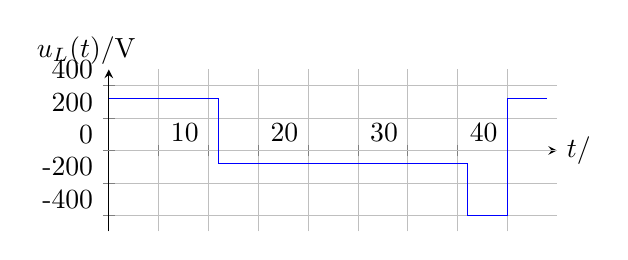
\begin{tikzpicture}
        \begin{axis}[
                domain=0:15,
                % x/y range adjustment
                xmin=0, xmax=45,
                ymin=-500, ymax=500,
                samples=500,
                axis y line=center,
                axis x line=middle,
                extra y ticks=0,
                % Label text
                xlabel={$t / \SI{}{\micro\second}$},,
                ylabel={$u_\text{L}(t)/\mathrm{V}$},
                % Label adjustment
                x label style={at={(axis description cs:1,0.5)},anchor=west},
                y label style={at={(axis description cs:-.05,.97)},anchor=south},
                width=0.6\textwidth,
                height=0.3\textwidth,
                % x-Ticks
                xtick={0,5,10,15,20,25,30,35,40},
                xticklabels={0,,10,,20,,30,,40},
                xticklabel style = {yshift=0.3cm,anchor=east},
                % y-Ticks
                ytick={400,200,0,-200,-400},
                yticklabels={400,200,,-200,-400},
                yticklabel style = {yshift=0.2cm,anchor=east},
                % Grid layout
                grid=both,
                grid style={line width=.1pt, draw=gray!10},
                major grid style={line width=.2pt,draw=gray!50},
            ]
            \addplot[color=blue,mark=none,solid] coordinates{
                (0, 320)
                (11, 320)
                (11, -80)
                (36, -80)
                (36, -400)
                (40, -400)
                (40, 320)
                (44, 320)
                };                
        \end{axis}
    \end{tikzpicture}
    \caption{Voltage at inductor in case 1.}
    \label{fig:VoltageAtInductorInCase1}
\end{solutionfigure}






    
    Case 2: With $U_\mathrm{1}$ = $\SI{720}{\volt}$ and $D_1 = 0.1$ you calculate the duty cycle $D_1$ by
    \begin{equation}
        D_1 = \frac{U_\mathrm{2}}{U_\mathrm{1}} \left(1 - D_2 \right)= \frac{\SI{400}{\volt}}{\SI{720}{\volt}} \cdot \left(1 - 0.1\right) = 0.5.
        \label{eq:DutyCycleD1}
    \end{equation}
    Again the inductor voltage is to calculate according \autoref{table:VoltageAtInductorInCase1_2}.
    The result is displayed in \autoref{fig:VoltageAtInductorInCase2}.

    %%%%%%%%%%%%%%%%%%%%%%%%%%%%%%%%%%%%%%%%%%%%%%%%%%%%%%%%%%%%%%%%%%%%%%%%%%
% VoltageAtInductorInCase2
%%%%%%%%%%%%%%%%%%%%%%%%%%%%%%%%%%%%%%%%%%%%%%%%%%%%%%%%%%%%%%%%%%%%%%%%%%

\begin{solutionfigure}[htb]
    \centering
    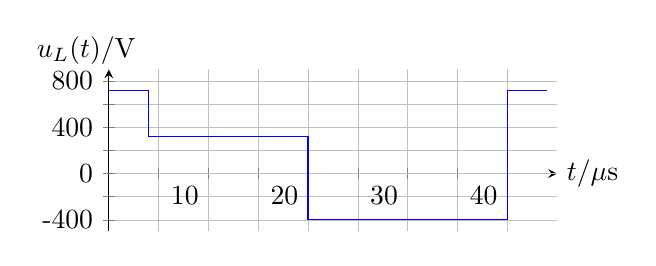
\begin{tikzpicture}
        \begin{axis}[
                domain=0:15,
                % x/y range adjustment
                xmin=0, xmax=45,
                ymin=-500, ymax=900,
                samples=500,
                axis y line=center,
                axis x line=middle,
                extra y ticks=0,
                % Labeltext
                xlabel={$t /\mathrm{\mu s}$},
                ylabel={$u_\text{L}(t)/\mathrm{V}$},
                % Label adjustment
                x label style={at={(axis description cs:1,0.36)},anchor=west},
                y label style={at={(axis description cs:-.05,.97)},anchor=south},
                width=0.6\textwidth,
                height=0.3\textwidth,,
                % x-Ticks
                xtick={0,5,10,15,20,25,30,35,40},
                xticklabels={0,,10,,20,,30,,40},
                xticklabel style = {yshift=-0.2cm,anchor=east},
                % y-Ticks
                ytick={800,600,400,200,0,-200,-400},
                yticklabels={800,,400,,,,-400},
                % Grid layout
                grid=both,
                grid style={line width=.1pt, draw=gray!10},
                major grid style={line width=.2pt,draw=gray!50},
            ]
            \addplot[color=blue,mark=none,solid] coordinates{
                (0, 720)
                (4, 720)
                (4, 320)
                (20, 320)
                (20, -400)
                (40, -400)
                (40, 720)
                (44, 720)
                };                 
        \end{axis}
    \end{tikzpicture}
    \caption{Voltage at inductor in case 2.}
    \label{fig:VoltageAtInductorInCase2}    
\end{solutionfigure}





        
\end{solutionblock}

\subtask{Calculate the voltage transformation ratio as a function of $D_1$ and $D_2$.}
\begin{solutionblock}
% Solution
    Based on equation \eqref{eq:DutyCycleD1} we easily solve to the voltage transformation ratio:
    \begin{equation}
        \frac{U_\mathrm{2}}{U_\mathrm{1}} \left(1 - D_2 \right) = D_1 
        \hspace{1cm} \Rightarrow \hspace{1cm}
        \frac{U_\mathrm{2}}{U_\mathrm{1}} = \frac{D_1} {1-D_2}.
    \end{equation}
\end{solutionblock}


\subtask{Express the current $I_\mathrm{L}$ as a function of the specified operating parameters
($U_\mathrm{1}$, $U_\mathrm{2}$, $P_\mathrm{2}$) and as a function of $D_\mathrm{1}$ and $D_\mathrm{2}$.}
\begin{solutionblock}
% Solution
    With the dependency of $I_\mathrm{L}$ from $I_\mathrm{2}$ and the duty cycle you get
    \begin{equation}
        I_\mathrm{L}=I_\mathrm{2} \frac{1}{1-D_2}= \frac{P_\mathrm{2}}{U_\mathrm{2}} \frac{1}{1-D_2}.
    \end{equation}.
\end{solutionblock}

\subtask{Are the calculated relationships valid if $T_1$ and $T_2$ do not switch synchronously or operate with
 different clock frequencies?}

\begin{solutionblock}
% Solution
    Yes, the relationsships are independent from the switching frequency and switching points.
\end{solutionblock}

\vspace{2em}\par
% Explaining text for the next subtask
If the transistors $T_1$ and $T_2$ are switched on, a constant voltage drop $U_\mathrm{F}=\SI{2.5}{\volt}$ occurs at the transistors
 regardless of the current. All other components are considered ideal and loss-free.

\subtask{How should $D_1$ and $D_2$ be selected so that the losses of the overall system are minimal?
 The relationships calculated under subtask 3.4 and 3.5 can be used for the voltage transformation ratio and the value of $I_\mathrm{L}$.}
\begin{solutionblock}
% Solution
    The losses of the transistors are to consider:
    \begin{equation}
        P_\mathrm{loss,T1}=D_1 U_\mathrm{F} I_\mathrm{L}=D_1 U_\mathrm{F} \frac{P_\mathrm{2}}{U_\mathrm{2}} \cdot \frac{1}{1-D_2}
        \hspace{1cm} \mathrm{and} \hspace{1cm}
        P_\mathrm{loss,T2}=D_2 U_\mathrm{F} I_\mathrm{L}=D_2 U_\mathrm{F} \frac{P_\mathrm{2}}{U_\mathrm{2}} \cdot \frac{1}{1-D_2}.
    \end{equation}
    So the losses of both transitors can be expressed by
    \begin{equation}
        P_\mathrm{loss}=\left(D_1 +D_2\right) U_\mathrm{F} \frac{P_\mathrm{2}}{U_\mathrm{2}} \cdot \frac{1}{1-D_2}
    \end{equation}
    and with
    \begin{equation}
        D_1 =\frac{U_\mathrm{1}}{U_\mathrm{2}} \left(1 - D_2 \right) 
        \hspace{1cm} \Rightarrow \hspace{1cm}
        P_\mathrm{loss}=\left(\frac{U_\mathrm{1}}{U_\mathrm{2}} \left(1 - D_2 \right)+D_2\right) U_\mathrm{F} \frac{P_\mathrm{2}}{U_\mathrm{2}} \cdot \frac{1}{1-D_2}.
    \end{equation}
    This leads to
    \begin{equation}
        P_\mathrm{loss}=P_\mathrm{2} U_\mathrm{F} \left(\frac{1}{U_\mathrm{1}} + 
        \frac{1}{U_\mathrm{2}} \cdot \frac{D_2}{1-D_2}\right).
        \label{eq:ploss}
    \end{equation}
    To minimize the losses depending on duty cycle you consider $P_\mathrm{loss}$=$f(D_2)$.
    \begin{equation}
        \frac{\mathrm{d}}{\mathrm{d}D_2} f(D_2)= \frac{1}{\left(1 - D_2 \right)^2}=0.
        \label{eq:derivateDutycyle}
    \end{equation}

    There is no solution in the real number space for equation \eqref{eq:derivateDutycyle}.
    If you consider \eqref{eq:ploss} the power loss decreases, when $\frac{D_2}{1-D_2}$ decrease.
    The following can be conclude from the result: \\
    $\Rightarrow$ Set $D_2$ as small as possible.\\
    $\Rightarrow$ Activate $T_2$ only for boost mode.\\
    $\Rightarrow$ Set $D_1$ as big as as possible.\\
\end{solutionblock}

\subtask{Plot $D_\mathrm{1}$ and $D_\mathrm{2}$ and the efficiency over $U_\mathrm{1}$ and give numerical values
 for $U_\mathrm{1} = \SI{320}{\volt}$, $U_\mathrm{1} = \SI{400}{\volt}$ and $U_\mathrm{1} = \SI{720}{\volt}$.}
\begin{solutionblock}
% Solution
    The power loss is to calculate with \eqref{eq:ploss} for the 3 different voltages.
    You get the efficiency by applying
    \begin{equation}
        \eta = \frac{P_\mathrm{2}}{P_\mathrm{loss}+P_\mathrm{2}}.
    \end{equation}
    With both equations you get the results according \autoref{table:PowerlossDutyCycleEfficiencyOpt}.
    This is displayed in \autoref{fig:DutyCycleOptAtInputVoltage}.

    %%%%%%%%%%%%%%%%%%%%%%%%%%%%%%%%%%%%%%%%%%%%%%%%%%%%%%%%%%%%%%%%%%%%%%%%%%
%  Minimal power loss, Duty cycles, power loss. efficiency 
%  depending on input voltage
%%%%%%%%%%%%%%%%%%%%%%%%%%%%%%%%%%%%%%%%%%%%%%%%%%%%%%%%%%%%%%%%%%%%%%%%%%

\begin{solutiontable}[ht]
    \centering  % Zentriert die Tabelle
    \begin{tabular}{lllll}
        \toprule
        \multicolumn{1}{c}{$U_\mathrm{1}$} & \multicolumn{1}{c}{$D$} & 
        \multicolumn{1}{c}{$D$} & \multicolumn{1}{c}{$P_\mathrm{loss}$} & 
        \multicolumn{1}{c}{$\eta_\mathrm{sync}$} \\
        \midrule 
        $U_\mathrm{1}$ & $D_1$   & $D_1$ & $P_\mathrm{loss}$      & $\eta_\mathrm{opt}$ \\ 
        $\SI{320}{\volt}$ & 1    & 0.2   & $\SI{46.88}{\watt}$ & 99.071 \\ 
        $\SI{400}{\volt}$ & 1    & 0     & $\SI{31.25}{\watt}$ & 99.379 \\ 
        $\SI{720}{\volt}$ & 0.56 & 0     & $\SI{17.36}{\watt}$ & 99.650 \\ 
        \bottomrule
    \end{tabular}
    \caption{Duty cycles, power loss and $\eta_\mathrm{opt}$ as fct. of $U_\mathrm{1}$.}
    \label{table:PowerlossDutyCycleEfficiencyOpt}  
\end{solutiontable}
    %%%%%%%%%%%%%%%%%%%%%%%%%%%%%%%%%%%%%%%%%%%%%%%%%%%%%%%%%%%%%%%%%%%%%%%%%%
% Dutycycle versus Input voltage
%%%%%%%%%%%%%%%%%%%%%%%%%%%%%%%%%%%%%%%%%%%%%%%%%%%%%%%%%%%%%%%%%%%%%%%%%%

\begin{solutionfigure}[htb]
    \centering
    \begin{tikzpicture}
        \begin{axis}[
                domain=0:15,
                xmin=300, xmax=820,
                ymin=0, ymax=1,
                samples=500,
                axis y line=center,
                axis x line=middle,
                % xtick distance=10,
                % ytick distance=100,
                extra y ticks=0,
                x label style={at={(axis description cs:1,0)},anchor=west},
                y label style={at={(axis description cs:-.05,.97)},anchor=south},
                width=0.6\textwidth,
                height=0.3\textwidth,
                xlabel={$U \text{[V]}$},
                ylabel={$D_(U_\mathrm{1})$},
                xtick={300,400,500,600,700,800},
                xticklabels={300,400,500,600,700,800},
                yticklabel style = {anchor=east,yshift=-0.2cm},
                grid=both,
                grid style={line width=.1pt, draw=gray!10},
                major grid style={line width=.2pt,draw=gray!50},
            ]
            \addplot[color=red,mark=none,solid] coordinates{
             (320, 1)
             (400, 1)
            };
            \addplot[signalred, domain=400:720] {400/x};
            \addplot[color=blue,mark=none,solid] coordinates{
             (400, 0)
             (720, 0)
            };
            \addplot[signalblue, domain=320:400] {1-(x/400)};
        \end{axis}
    \end{tikzpicture}
    \caption{Duty cycle versus input voltage.}
\end{solutionfigure}







    
\end{solutionblock}

\subtask{Calculate the efficiency for the three operating points in subtask 3.2.}

\begin{solutionblock}
% Solution
    Again the equation \eqref{eq:ploss} is used with the condition $D_1$=$D_2$=$D$. This leads to
    \begin{equation}
        P_\mathrm{loss}=2D U_\mathrm{F} I_\mathrm{L} = \frac{U_\mathrm{f} P_\mathrm{2}}{U_\mathrm{2}} \cdot \frac{2D}{1-D}
    \end{equation}
    If you enter the 3 operation voltages you get the results according \autoref{table:PowerlossDutyCycleEfficiencySync}.
    %%%%%%%%%%%%%%%%%%%%%%%%%%%%%%%%%%%%%%%%%%%%%%%%%%%%%%%%%%%%%%%%%%%%%%%%%%
%  power loss, Duty cycles, power loss. efficiency 
%  depending on input voltage at synchron mode
%%%%%%%%%%%%%%%%%%%%%%%%%%%%%%%%%%%%%%%%%%%%%%%%%%%%%%%%%%%%%%%%%%%%%%%%%%

\begin{solutiontable}[ht]
    \centering  % Zentriert die Tabelle
    \begin{tabular}{lllll}
        \toprule
        
        $U_\mathrm{1}$ & $D_1$   &  $D_1$ & $P_\mathrm{loss}$      & $\eta_\mathrm{sync}$ \\ 
        $\SI{320}{\volt}$ & 0.56 &  0.56  & $\SI{78.12}{\watt}$ & 98.462 \\ 
        $\SI{400}{\volt}$ & 0.5  &  0.5   & $\SI{62.50}{\watt}$ & 98.765 \\ 
        $\SI{720}{\volt}$ & 0.36 &  0.36  & $\SI{35.16}{\watt}$ & 99.300 \\ 
        \bottomrule
    \end{tabular}
    \caption{$Dutycycles$, power loss and $\eta_\mathrm{sync}$ as fct. of $U_\mathrm{1}$.}     
\end{solutiontable}

    
\end{solutionblock}

\subtask{How high is the maximum efficiency gain and at which operating point does it occur? Give an explanation
 for the observed finding.}

\begin{solutionblock}
% Solution
    The efficiency gain is calculated by $\Delta \eta$=$\eta_\mathrm{opt}$-$\eta_\mathrm{sync}$.
    You get following result:

    \begin{table}[ht]
    \centering  % Zentriert die Tabelle
    \begin{tabular}{lllll}
        \toprule
        
        $U_\mathrm{1}$ & $\Delta\eta$ \\ 
        $\SI{320}{\volt}$ & 0.609 \\ 
        $\SI{400}{\volt}$ & 0.614  \\ 
        $\SI{720}{\volt}$ & 0.350 \\ 
        \bottomrule
    \end{tabular}
\end{table}
    
    The maximum efficiency gain is at $U_\mathrm{1}=\SI{400}{\volt}$. \\
    It looks like the efficiency gain is higher within boost mode,
     but why is the highest efficiency gain at $\SI{400}{\volt}$? \\
    Let's consider the power loss at boost mode for the two cases. The power loss needs to be expressed by a function of the voltages:

    \begin{equation}
        P_\mathrm{loss}=D_1 U_\mathrm{F} I_\mathrm{L} + D_2 U_\mathrm{F} I_\mathrm{L}.
        \label{eq:ploss2}
    \end{equation}
    If following is considered
    \begin{equation}
        I_\mathrm{L}=\frac{P_\mathrm{2}}{U_\mathrm{1}} 
        \hspace{1cm} \mathrm{and} \hspace{1cm}
        D_1=1
        \hspace{1cm} \mathrm{and} \hspace{1cm}
        D_2=1-\frac{U_\mathrm{1}}{U_\mathrm{2}} 
    \end{equation}
    this leads to
    \begin{equation}
        P_\mathrm{loss,opt}=\frac{2 P_\mathrm{2} U_\mathrm{F}}{U_\mathrm{1}} - \frac{P_\mathrm{2} U_\mathrm{F}}{U_\mathrm{2}}.
    \end{equation}

    For the synchronous operation mode following is valid:
    consider:
    \begin{equation}
        I_\mathrm{L}=\frac{P_\mathrm{2}}{U_\mathrm{2}} \cdot \frac{1}{1-D}  
        \hspace{1cm} \mathrm{and} \hspace{1cm}
        D_1=D_2=D
        \hspace{1cm} \mathrm{and} \hspace{1cm}
        D=\frac{U_\mathrm{2}}{U_\mathrm{1}+U_\mathrm{2}}.
    \end{equation}
    With \eqref{eq:ploss2} this leads now to
    \begin{equation}
        P_\mathrm{loss,sync}=\frac{P_\mathrm{2} U_\mathrm{F}}{U_\mathrm{1}} + \frac{P_\mathrm{2} U_\mathrm{F}}{U_\mathrm{1}}=\frac{2 P_\mathrm{2} U_\mathrm{F}}{U_\mathrm{1}}.
    \end{equation}

    The efficiency can be expressed by 
    \begin{equation}
        \eta = \frac{P_\mathrm{2}}{P_\mathrm{loss}+P_\mathrm{2}}=\frac{1}{1+\frac{P_\mathrm{loss}}{P_\mathrm{2}}}.
    \end{equation}
    If the result of the power losses is inserted into the formula, you get:
    \begin{equation}
        \eta_\mathrm{opt} = \frac{1}{1+U_\mathrm{F} \left(\frac{2}{U_\mathrm{1}}-\frac{1}{U_\mathrm{2}}\right)}
        \hspace{1cm} \mathrm{and} \hspace{1cm}
        \eta_\mathrm{sync} = \frac{1}{1+U_\mathrm{F} \frac{2}{U_\mathrm{1}}}.
        \label{eq:efficiencies}
    \end{equation}

    The minimal efficiency gain is the minimum of $\Delta \eta=\eta_\mathrm{opt}-\eta_\mathrm{sync}$.
    
    \begin{equation}
        \Delta \eta= \frac{\frac{U_\mathrm{F}}{U_\mathrm{2}}}{\left(1+ \frac{2 U_\mathrm{F}}{U_\mathrm{1}}-\frac{U_\mathrm{F}}{U_\mathrm{2}} \right) \left(1+\frac{2 U_\mathrm{F}}{U_\mathrm{1}}\right)}.
    \end{equation}

    The two efficiencies are calculated with \eqref{eq:efficiencies} and displayed in \autoref{fig:EfficiencyAtInputVoltage}.
    %%%%%%%%%%%%%%%%%%%%%%%%%%%%%%%%%%%%%%%%%%%%%%%%%%%%%%%%%%%%%%%%%%%%%%%%%%
% Efficiency versus Input voltage
%%%%%%%%%%%%%%%%%%%%%%%%%%%%%%%%%%%%%%%%%%%%%%%%%%%%%%%%%%%%%%%%%%%%%%%%%%

\begin{solutionfigure}[htb]
    \centering
    \begin{tikzpicture}
        \begin{axis}[
                %domain=0:15,
                xmin=300, xmax=820,
                ymin=98, ymax=100,
                samples=500,
                axis y line=center,
                axis x line=middle,
                extra y ticks=0,
                x label style={at={(axis description cs:1,0)},anchor=west},
                y label style={at={(axis description cs:-.05,.97)},anchor=south},
                width=0.6\textwidth,
                height=0.3\textwidth,
                xlabel={$U \text{[V]}$},
                ylabel={Efficiency $[\%]$},
                ylabel style = {yshift=0.2cm},
                xtick={300,400,500,600,700,800},
                xticklabels={300,400,500,600,700,800},
                yticklabel style = {anchor=east},
                grid=both,
                grid style={line width=.1pt, draw=gray!10},
                major grid style={line width=.2pt,draw=gray!50},
            ]
            \addplot[signalred, domain=320:720] {100/(1+(2.5*2/x))};
            \addplot[signalblue, domain=320:720] {100/(1+(2.5*((2/x)-(1/400))))};
        \end{axis}
    \end{tikzpicture}
    \caption{Duty cycle versus input voltage.}
\end{solutionfigure}









    Conclusion: \\
    $\Rightarrow$ You get the minimal efficiency gain at maximal $U_\mathrm{1}$. \\
    $\Rightarrow$ The difference between the power losses of $P_\mathrm{loss,opt}$ and $P_\mathrm{loss,sync}$ in boost mode is the constant factor 
    $\frac{P_\mathrm{2} U_\mathrm{F}}{U_\mathrm{2}}$
    which has a proportionally greater effect on the efficiency with smaller $U_\mathrm{2}$ power losses (here larger $U_\mathrm{1}$ ).

\end{solutionblock}
